\documentclass[]{article}
\usepackage[dutch]{babel}
\usepackage{graphicx}
\usepackage{amsmath}
\usepackage[]{siunitx}
\usepackage{hyperref}
\usepackage{booktabs}
%opening
\title{Lab: Embedded system design 1}
\author{Thomas Feys \and Jona Cappelle}

\begin{document}

\maketitle

\newpage

\tableofcontents

\newpage

\section{Inleiding}
Ons doel is om de wachtrij in de rabotaria te monitoren. Dit zullen we doen aan de hand van een IR grid sensor (AMG8833). Aan de hand van de uitgelezen waarden zullen we in het tweede semester bepalen hoeveel mensen er in de wachtrij staan. Deze informatie zullen we vervolgens via een app of website verspreiden.


\section{Sensor}
De sensor die we gebruiken om de wachtrij te monitoren is de AMG8833. Deze IR grid sensor heeft 8x8 pixels die de temperatuur weergeven. Volgens de datasheet kan a.d.h.v. de temperatuur een mens waargenomen worden vanop een afstand van 5 meter. De sensor kan gebruikt worden in 3 verschillende modes: normal, sleep en stand-by. In de normale mode heeft de sensor een verbruik van 4.5 mA. De stand-by mode heeft twee opties; de waardes kunnen geüpdatet worden om de 60 seconden of om de 10 seconden. In deze mode is er een verbruik van 0.8 mA. Als laatste is er de sleep mode deze verbruikt 0.2 mA. Een overzicht van alle modes en de commando's die verstuurd moeten worden om in deze modes te gaan, wordt weergegeven in figuur \ref{fig:operatingmodes}. Tijdens het testen van de sensor hebben we periodiek geswitched tussen de verschillende power modes. Het resultaat van deze test is te zien in figuur \ref{fig:powertest}. De sensor heeft ook een interrupt pin. Deze pin geneert een interrupt als een van de pixels over of onder een bepaalde waarde gaat. Deze waarde is instelbaar.	
\begin{figure}[!ht]
	\centering
	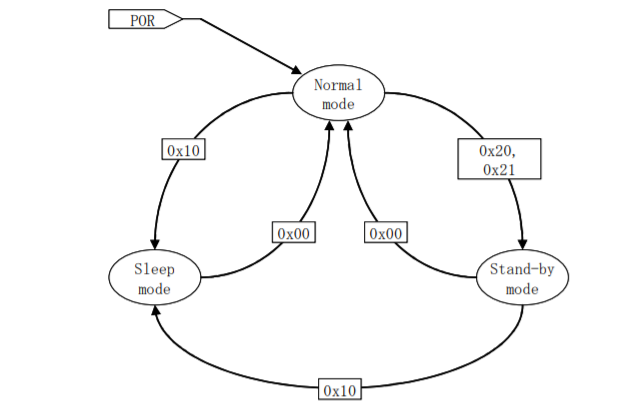
\includegraphics[width=\columnwidth]{operatingmodes.png}
	\caption{Overzicht operating modes}
	\label{fig:operatingmodes}
\end{figure}

%todo figuur aanpassen naar screenshot powermodes in de power monitor 
%todo test doen in verschillende modes met processor in sleep

\begin{figure}[!ht]
	\centering
	\includegraphics[width=\columnwidth]{power_modes_cycle_AMG8833_em2.png}
	\caption{Test van de verschillende powermodes}
	\label{fig:powertest}
\end{figure}

\section{Systeem}
\subsection{Overzicht}
De AMG8833 communiceert met de EFM32 via I2C. Naast de I2C communicatie is er ook een interrupt pin voorzien op de sensor. Deze pin genereert een interrupt als er een van de pixels een bepaalde, instelbare waarde overschrijdt. Een volledig overzicht van het systeem is te zien in figuur \ref{fig:systeem}.

\begin{figure}[!ht]
	\centering
	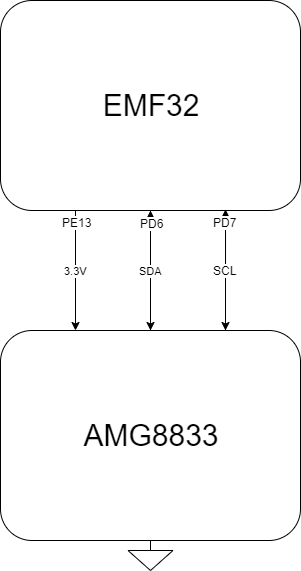
\includegraphics[scale=0.5]{sys1.png}
	\caption{Overzicht van het systeem}
	\label{fig:systeem}
\end{figure}
\subsection{I2C}
De communicatie met de sensor gebeurt via I2C. Het adres van de sensor is een 7 bit adres namelijk: 1101001. Aangezien we met een 7 bit adres zitten moet deze 1 bit geshift worden naar links. Dit adres moet telkens naar de sensor verstuurd worden vooraleer er iets gelezen of geschreven kan worden. De code die gebruikt wordt om de sensor uit te lezen, in andere powermodus te zetten en te interrupten wordt in de volgende sectie besproken. 


\section{Code}
\subsection{Functionaliteiten}
Om gemakkelijk met de sensor te werken werd er een library geschreven voor de AMG8833. Er werden verschillende methodes geschreven om vlot te kunnen omgaan met de sensor. Er werd een functie geschreven om alle pixels uit te lezen. Naast de pixels is er ook een thermistor aanwezig in de sensor, ook hiervoor werd een functie geschreven. Er werden ook verschillende functies geschreven om makkelijk tussen de verschillende powermodes te kunnen wisselen. Een volledig overzicht van deze library en de rest van de code is terug te vinden op github: \url{https://github.com/jonacappelle/Embedded_Project}.


\subsection{Flow van de code}
\label{flowcode}
Aangezien de sensor in stand-by een verbruik van 0.8~mA heeft wordt deze altijd in sleep gezet. De sensor wordt om de 5 minuten uit sleep gehaald om alle pixels uit te lezen. Hierna wordt ze weer in sleep gezet. Een volledig overzicht van de code is terug te vinden in figuur \ref{fig:flowchart}.

\begin{figure}[!ht]
	\centering
	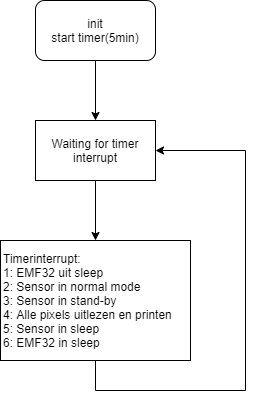
\includegraphics[scale=0.5]{flowchart.png}
	\caption{flowchart van de code}
	\label{fig:flowchart}
\end{figure}


\section{Power consumptie}
\subsection{Sensor}
De sensor heeft 3 verschillende powermodes, deze zijn te zien in figuur \ref{fig:sensor_power}. Deze hebben we ook zelf opgemeten zoals te zien is in figuur \ref{fig:powertest}. De gemeten waarden liggen in dezelfde grote orde als deze die opgegeven zijn in de datasheet, maar wijken toch een klein beetje af. In normal mode gebruikt onze sensor 4.95~mA, in stand-by 0.66~mA en in sleep  0.156~mA.

\begin{figure}[!ht]
	\centering
	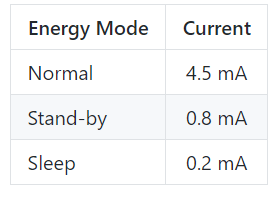
\includegraphics{sensor_power.png}
	\caption{powermodes van de sensor}
	\label{fig:sensor_power}
\end{figure}

\subsection{Principe}
\paragraph{Sensor: }
Door de methode toe te passen die besproken werd in section \ref{flowcode} wordt de power consumptie sterk verminderd. De sensor zit enkel in stand-by tijdens het uilezen van de sensor waarde. De sensor zit ook 105~ms in normal mode, omdat je altijd naar de normal mode moet gaan als je uit sleep komt. Er werd een meting uitgevoerd om dit verbruik te controleren, dit is terug te vinden in figuur \ref{fig:meting}. Uit deze meting is te zien dat de sensor 105~ms in normal mode zit met een verbruik van 4.8~mA, 50ms in stand-by met een verbruik van 2.83~mA\footnote{Tijdens het uitlezen van de sensor ligt het verbruik hoger, hierdoor verbruikt de sensor 2.83~mA in stand-by ipv 0.8~mA} en verder zit de sensor in sleep met een verbruik van 0.156~mA. Hierdoor bekomen we volgend verbruik per meting:
\begin{equation}
	 3.3\text{ V}\cdot\big(105\text{ ms} \cdot 4.8 \text{ mA} + 50\text{ ms}\cdot 2.83\text{ mA}+299.845\text{ s}\cdot 0.156\text{ mA}\big) = 156.4904 \text{ mJ/meting}
\end{equation}
Een overzicht is te zien in tabel \ref{tab:verbruik}.


% Please add the following required packages to your document preamble:
% \usepackage{booktabs}
% \usepackage{graphicx}
\begin{table}[h!]
	\centering
	%\resizebox{\textwidth}{!}{%
	\begin{tabular}{@{}llll@{}}
	\toprule
	Power Mode & Verbruik {[}mA{]} & Tijd {[}s{]} & Energie {[}mJ{]} \\ \midrule
	Normal     & 4.8               & 0.105        & 1.6632           \\
	Stand-By   & 2.83              & 50           & 0.4669           \\
	Sleep      & 0.156             & 299.845      & 154.3602         \\
			   &                   & Totaal       & 156.4904         \\ \bottomrule
	\end{tabular}%
	%}
	\caption{Verbruik voor \'e\'en meting}
	\label{tab:verbruik}
	\end{table}



Als we om de 5 minuten een meting uitvoeren, bekomen we volgend verbruik:
\begin{align*}
	12\cdot 156.4904 \dfrac{\text{mJ}}{\text{meting}} &=  \SI{1.877}{mJ} \\
	\Rightarrow \dfrac{1.877\text{ J}}{3600\text{ s}} &= \SI{0.52}{mW}
\end{align*}




In plaats van een constant verbruik van 0.8~mA verbrverbruikt de sensor maar 0.2~mA aangezien hij bijna constant in sleep zit. Het verbruik zal een klein beetje hoger zijn aangezien de sensor voor een kleine tijd weer in normal en stand-by mode gezet wordt. 
\paragraph{Processor: }
De processor wordt enkel uit sleep gehaald als er een timerinterrupt afgaat. Hierdoor zit de processor voornamelijk in EM2 dit geeft een verbruik van 0.9~$\mu$A.


\begin{figure}[h!]
	\centering
	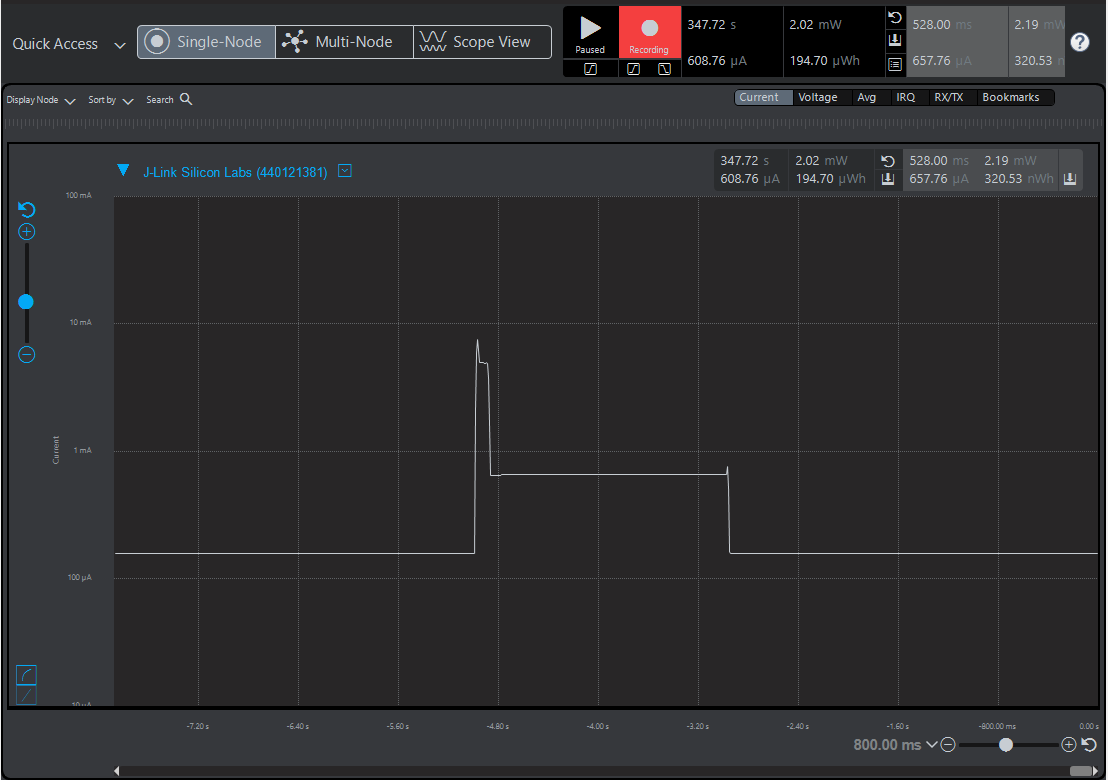
\includegraphics[width=\columnwidth]{final_energy_consumption.png}
	\caption{Meting verbruik}
	\label{fig:meting}
\end{figure}





\newpage

\section{Besluit }



\end{document}
